% ------------------------------------------------------------------------ %
% !TEX encoding = UTF-8 Unicode
% !TEX TS-program = pdflatex
% !TEX root = ../Tesi.tex
% !TEX spellcheck = it-IT
% ------------------------------------------------------------------------ %
%
% ------------------------------------------------------------------------ %
% 	NOME APPENDICE 1
% ------------------------------------------------------------------------ %
%
\chapter{Block Header Ethereum}
%
\label{cap:blockheader}
%
\begin{figure}[H]
	%
	\centering
	%
	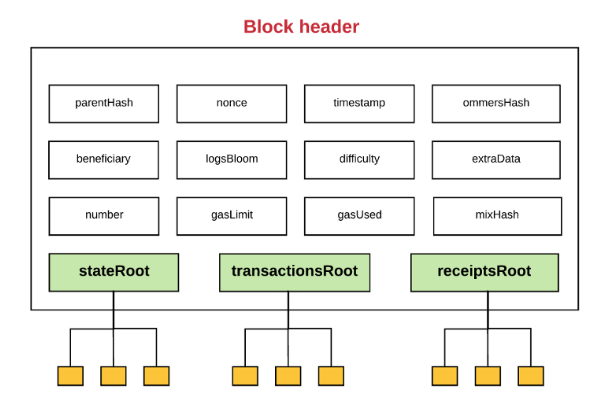
\includegraphics[width=.8\textwidth]{Ethereum/blockHeader}
	%
	\caption{Schema Blocco in Ethereum}
	%
	\label{fig:schema blocco in Ethereum}
	%
\end{figure}
In ethereum un blocco è composto da:
\begin{itemize}
	\item il block header;
	\item le informazioni che riguardano l'insieme delle transazioni incluse nel blocco;
	\item un insieme di altri block header per l'attuale block ommers. Con \enquote*{ommer} o \enquote*{uncle block} si intende un figlio di un antenato che non è un antenato. Se A è uncle di B, B è nipote di A. Questi sono necessari per aiutare a ricompensare i miners quando sono trovate soluzioni duplicate di blocchi a causa dei tempi di blocco più corti di Ethereum (rispetto a Bitcoin ad esempio). Un uncle è una ricompensa più piccola rispetto ad un full block (se sono inviati oltre il blocco successivo, la ricompensa decresce rapidamente fino a zero dopo sette blocchi).
\end{itemize}%
La parte che contiene la maggior parte delle informazioni per il corretto funzionamento della blockchain è il block header. Esso è composto da:
\begin{enumerate}
	\item parentHash: l'\gls{hash} del block header genitore (questo è quello che rende l'insieme di blocchi una catena);
	\item ommersHash: l'hash della corrente lista di block ommers;
	\item beneficiary: l'indirizzo dell'account che riceve la ricompensa per minare il blocco;
	\item stateRoot: struttura dati di tipo Tree. Contiene l'hash del root node dello state tree (così è facile per i light client verificare gli stati);
	\item transactionsRoot: struttura dati di tipo Tree. Contiene l'hash del root node del tree che contiene tutte le transazioni listate nel blocco;
	\item receiptsRoot: struttura dati di tipo Tree. Contiene l'hash del root node del tree che contiene le ricevute di tutte le transazioni listate nel blocco;
	\item logsBloom: una struttura dati che contiene informazioni di log;
	\item difficulty: indica il livello di difficoltà del blocco;
	\item number: il numero del blocco corrente (il genesis block ha numero di blocco 0);
	\item gasLimit: l'attuale gasLimit per blocco;
	\item gasUsed: la somma del gas totale usato dalle transazioni in questo blocco;
	\item timestamp: iltimestamp unix dell'inception di questo blocco;
	\item extraData: dati extra relativi a questo blocco;
	\item mixHash: un hash che, quando combinato con il nonce, dimostra che questo blocco ha portato avanti sufficiente computazione;
	\item nonce: un hash che, quando combinato con il mixHash, dimostra che questo blocco ha portato avanti sufficiente computazione.
\end{enumerate}%
